\section{Experiments}\label{sec:Experiments}
In this section, we empirically study the behavior of $1$-GNNs, $2$-GNNs, and $3$-GNNs on the problem of distinguishing graphs that contain a $k$-clique from graphs that are $(k\!-\!1)$-colorable. We evaluate both training and test performance, using the former to assess how well the models fit the task and the latter to measure their ability to generalize.

We evaluate the three GNN architectures under three different experimental settings. In Experiment~1, we train and test the models on \emph{implanted random graphs}: random $N$-vertex graphs generated either by planting a $k$-clique, or by imposing a $(k\!-\!1)$-partition in which each color class forms an independent set and edges are added independently across classes. In Experiment~2, we modify this data-generation procedure so that the two graph classes have matching average degree (this adjustment is described in detail in Subsection~\ref{subsec:DataGeneration}). In Experiment~3, we evaluate the models on the hard graph family $\Fam_k$ introduced in Section~\ref{sec:HardFamilies}.


\subsection{Dataset generation}\label{subsec:DataGeneration}

We consider three different data-generation procedures corresponding to the experimental settings described above.

\textbf{Implanted random graphs.}\todo{Justify/motivate/add references on planted clique graphs and fixed random color class graphs.} 
In the first experimental setting, graphs are generated uniformly at random from two classes: graphs on $N$ vertices that contain a $k$-clique, and graphs on $N$ vertices that are $(k\!-\!1)$-colorable. Both classes are generated using Erd\H{o}s--R\'enyi-style random constructions with edge probability $p=0.5$. In particular, $(k\!-\!1)$-colorable graphs are generated by randomly partitioning the vertex set into $(k\!-\!1)$ parts and independently adding edges between vertices in different parts with probability $0.5$, while $k$-clique graphs are generated by first planting a $k$-clique and then adding all remaining edges independently at random with probability $0.5$. As node features, we use the degree of each vertex.

Due to structural differences between graphs generated by the two generation procedures, the resulting graphs naturally exhibit markedly different average degrees.
In particular, graphs containing a $k$-clique tend to have higher average degree than $(k\!-\!1)$-colorable graphs. %This can be shown analytically.

% \begin{observation}[Expected average degree gap in Experiment~1]
% \label{obs:avg-degree-gap}
% Fix $N \in \N$ and $k \ge 3$, and let $p=0.5$.
% \begin{enumerate}
%     \item (\emph{$(k\!-\!1)$-colorable graphs.})
%     Generate a random $(k\!-\!1)$-colorable graph by partitioning $V$ uniformly at random into $(k\!-\!1)$ parts and then adding each edge between different parts independently with probability $p$.
%     Then the expected average degree satisfies
%     \[
%     \E[d_{\avg}] \;=\; p\,(N-1)\frac{k-2}{k-1}
%     \;=\; \frac{1}{2}(N-1)\frac{k-2}{k-1}.
%     \]
%     \item (\emph{Graphs with a planted $k$-clique.})
%     Generate a random graph with a planted $k$-clique by first selecting a $k$-subset $S \subseteq V$ and adding all edges inside $S$, and then adding every remaining edge independently with probability $p$.
%     Then the expected average degree satisfies
%     \[
%     \E[d_{\avg}]
%     \;=\;
%     \frac{k(N-1) + (N-k)(N-k-1)}{N}.
%     \]
% \end{enumerate}
% In particular, for $N>k$ one has $\E[d_{\avg}]$ larger in the planted-$k$-clique model than in the $(k\!-\!1)$-colorable model, yielding an explicit average-degree gap.
% \end{observation}


\begin{figure}[h]
    \centering
    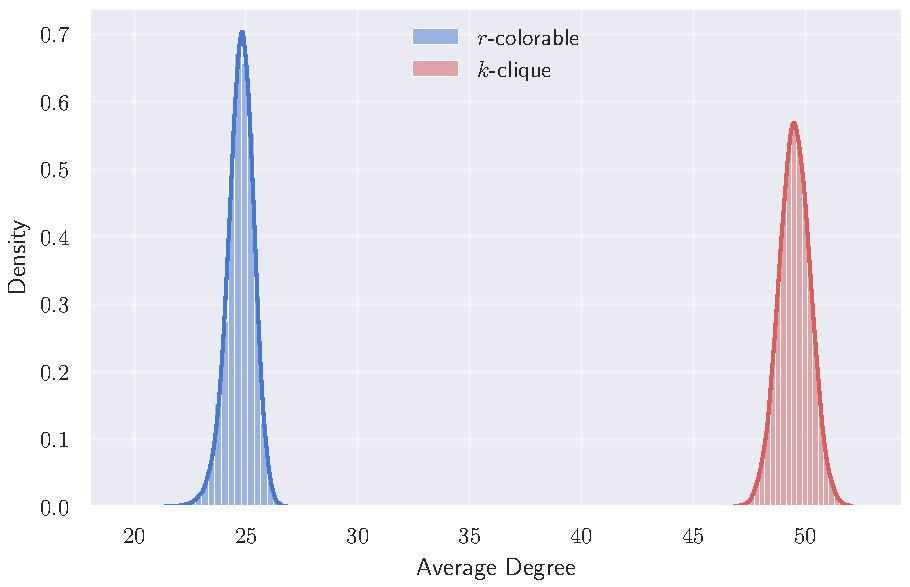
\includegraphics[width=0.9\linewidth]{sketches/plots/same-edgeprob.pdf}
    \caption{Histogram with KDE of average degrees for 2-colorable and 3-clique graphs with $N = 100$ and $p = 0.5$}
    \label{fig:avg-degrees}
\end{figure}

As a consequence, the two classes can often be separated by simple statistics such as average degree, making this setting comparatively easy for graph neural networks. %(This is discussed in more detail in section \ref{subsec:ResultsandDiscussion}). 
This observation immediately motivates a more constrained experimental setting.


\textbf{Matching average degree.}
To eliminate trivial separation y degree, the second experimental setting modifies the data-generation process so that the two graph classes have matching expected average degree. This is achieved by adjusting the edge probability in the random construction of the $k$-clique graphs so that their expected average degree coincides with that of the $(k\!-\!1)$-colorable graphs. 
The average degree of clique implanted graphs is given by,

\begin{equation}
\label{eq:r-edgeprob}
    \begin{split}
        d_{avg} = p(n-1)\frac{(r-1)}{r}
    \end{split}
\end{equation}

while the average degree of $n$-node color class implanted graphs is given by. 

\begin{equation}
\label{eq:s-edgeprob}
    \begin{split}
        d_{avg} = \frac{s(s-1) + q(n-s) s  +2q (n -s) (n-s-1) }{n}
    \end{split}
\end{equation}

Combining equations \ref{eq:r-edgeprob} and \ref{eq:s-edgeprob} gives a probability $p$ generating clique implanted graphs and color class implanted graphs with matching average (expected) degrees. 
As a result, the empirical degree distributions of the two classes become nearly indistinguishable, while the underlying clique versus coloring structure is preserved (see figure \ref{fig:same-dist}). 

\begin{figure}[htbp]
    \centering
    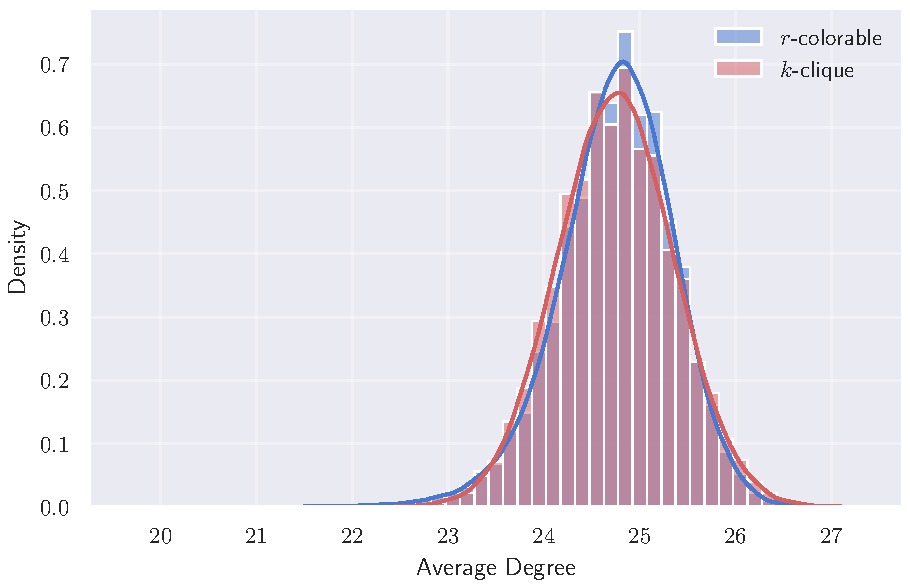
\includegraphics[width=0.9\linewidth]{sketches/plots/same-dist.pdf}
    \caption{Histogram with KDE of average degrees for 2-colorable and 3-clique graphs with $N = 100$ and edge probability adjusted to give the same average degree.}
    \label{fig:same-dist}
\end{figure}

This setting controls for degree-based heuristics and provides a more challenging benchmark for assessing whether GNNs can learn more subtle structural features.

\textbf{Hard graph family.}
In the third experimental setting, we evaluate the models on the explicit hard graph family $\Fam_k$ introduced in Section~\ref{sec:HardFamilies}.


\subsection{Models and configurations}\label{sec:ModelsandConfig}
We use standard off the shelf GCN models from 


\subsection{Results and Discussion}\label{subsec:ResultsandDiscussion}
The results from experiment 1 indicate that in general the $k$-clique vs $(k-1)$-colorable classification task is easy for even standard of the shelf GNNs.

\textbf{Training performance.}

\textbf{Test performance.}


\newpage